\documentclass[boxes,pages]{homework}

\name{Nate Stemen}
\studentid{20906566}
\email{nate.stemen@uwaterloo.ca}
\term{Fall 2020}
\course{Numerical Analysis}
\courseid{AMATH 740}
\hwnum{2}
\duedate{Fri, Sep 25, 2020 5:00 PM}

\hwname{Assignment}


\usepackage{physics}
% \usepackage[makeroom,Smaller]{cancel}
\usepackage{cleveref}
\usepackage{marginnote}
% \usepackage{tikz}
% \usetikzlibrary{arrows}
\usepackage{tkz-euclide}
\renewcommand*{\marginfont}{\footnotesize}

\newcommand{\tpose}[1]{#1^\intercal}
\newcommand{\inv}[1]{#1^{-1}}

\DeclareMathOperator{\fl}{fl}


\begin{document}

\begin{problem}
Floating point numbers.
\end{problem}

\begin{solution}
	It's helpful if we start with a picture. Let $\alpha, \beta$ be two adjacent numbers in our number system and $x$ to be equidistant between them.
	\begin{center}
		\begin{tikzpicture}
			\draw[latex-] (-3,0) -- (3,0) ;
			\draw[-latex] (-3,0) -- (3,0) ;
			\foreach \x in {-2,0,2} {
					\draw[shift={(\x,0)},color=black] (0pt,3pt) -- (0pt,-3pt);
				}
			\draw[shift={(-2,0)},color=black] (0pt,0pt) -- (0pt,-3pt) node[below]{$\alpha$};
			\draw[shift={(2,0)},color=black] (0pt,0pt) -- (0pt,-3pt) node[below]{$\beta$};
			\draw[shift={(0,0)},color=black] (0pt,0pt) -- (0pt,-3pt) node[below]{$x$};
		\end{tikzpicture}
	\end{center}
	Note if we round $x$ as $\fl(x)$, then $x$ will be rounded to either $\alpha$ or $\beta$ depending on even-ness. By the definition of floating point number systems, the distance between $\alpha$ and $\beta$ is $\beta^{-t + 1}$ ($\alpha - \beta = \beta^{-t + 1}$), and because the way we positioned $x$ we have $x = \alpha + \frac{1}{2}\beta^{-t + 1} = \alpha + \mu$. If we take $\alpha = 1$ and $\beta = 1 + \texttt{eps}$, then we can see the distance between them is $2\mu$ and hence $\texttt{eps} = 2\mu$.
\end{solution}

\begin{problem}
Consider the expression
\[
	z_A = \frac{1}{\sqrt{1 + x^2} - \sqrt{1 - x^2}}.
\]
\begin{parts}
	\part{Explain why the formula for $z_A$ is susceptible to catastrophic cancellation errors for $x$ close to 0.}\label{part:2a}
	\part{Use reformulation to find an alternative expression $z_B$ for expression $z_A$ in a way that avoids catastrophic cancellation for $x$ close to 0. (Hint: $p^2 - q^2 = (p - q)(p + q)$.)}\label{part:2b}
\end{parts}
\end{problem}

\begin{solution}
	\ref{part:2a}
	To see why $z_A$ is susceptible to catastrophic cancellation we can use the Taylor expansion around $x = 0$ of $\sqrt{1 + x} \approx 1 + \frac{x}{2}$.
	\begin{align*}
		z_A & = \frac{1}{\sqrt{1 + x^2} - \sqrt{1 - x^2}}                 \\
		    & \approx \frac{1}{1 + \frac{1}{2}x^2 - (1 - \frac{1}{2}x^2)}
	\end{align*}
	Just as we saw in lecture, when subtracting two numbers that are very close to each other (in this case $1 + \varepsilon$ and $1 - \varepsilon$), then we are susceptible to catastrophic cancellation.

	\ref{part:2b}

	In order to avoid catastrophic cancellation we can further the last line of $z_A$ to express it as $\frac{1}{x^2}$. Written this was there is no catastrophic cancellation, just a blowup at $x = 0$.
\end{solution}

\begin{problem}
Consider the matrix
\[
	A = \mqty[2 & 0 & 0 \\ 0 & 1 & 1 \\ 0 & 1 & 2 \\ 0 & 0 & 0]\in\mathbb{R}^{4\times 3}
\]
\begin{parts}
	\part{Determine (by hand) the reduced $QR$ factorization of $A$ using the Gram-Schmidt algorithm. I.e., orthonormalise the column vectors of $A$, and write the result as \[A = \widehat{Q}\widehat{R},\] with $\widehat{Q}\in\mathbb{R}^{4\times 3}$ and $\widehat{R}\in\mathbb{R}^{3\times 3}$.}\label{part:3a}
	\part{Extend this to the full $QR$ factorization of $A$:\[ A = QR \] with $Q\in\mathbb{R}^{4\times 4}$ and $R\in\mathbb{R}^{4\times 3}$.}\label{part:3b}
\end{parts}
\end{problem}

\begin{solution}
	\ref{part:3a}
	This is mostly a computational question, so I'll just show that.
	\begin{align*}
		\vb{u}_1 & = \vb{a}_1 =  \mqty[2 \\ 0 \\ 0 \\ 0] & \vb{e}_1 & = \mqty[1 \\ 0 \\ 0 \\ 0] \\
		\vb{u}_2 & = \vb{a}_2 - \frac{\langle\vb{u}_1, \vb{a}_2\rangle}{\langle\vb{u}_1, \vb{u}_1\rangle}\vb{u}_1 = \mqty[0 \\ 1 \\ 1 \\ 0] & \vb{e}_2 & = \frac{1}{\sqrt{2}}\mqty[0 \\ 1 \\ 1 \\ 0] \\
		\vb{u}_3 & = \vb{a}_3 - \frac{\langle\vb{u}_1, \vb{a}_3\rangle}{\langle\vb{u}_1, \vb{u}_1\rangle}\vb{u}_1 - \frac{\langle\vb{u}_2, \vb{a}_3\rangle}{\langle\vb{u}_2, \vb{u}_2\rangle}\vb{u}_2 =  \frac{1}{2}\mqty[0 \\ -1 \\ 1 \\ 0] & \vb{e}_3 & = \frac{1}{\sqrt{2}}\mqty[0 \\ -1 \\ 1 \\ 0]
	\end{align*}
	We can then construct the reduced factorization as follows.
	\begin{align*}
		\widehat{Q} & = \mqty[\vb{e}_1 & \vb{e}_2 & \vb{e}_3] = \mqty[1 & 0 & 0 \\ 0 & \frac{1}{\sqrt{2}} & \frac{-1}{\sqrt{2}} \\ 0 & \frac{1}{\sqrt{2}} & \frac{1}{\sqrt{2}} \\ 0 & 0 & 0] \\
		\widehat{R} & = \mqty[\langle\vb{e}_1,\vb{a}_1\rangle & \langle\vb{e}_1,\vb{a}_2\rangle & \langle\vb{e}_1,\vb{a}_3\rangle \\ 0 & \langle\vb{e}_2,\vb{a}_2\rangle & \langle\vb{e}_2,\vb{a}_3\rangle \\ 0 & 0 & \langle\vb{e}_3,\vb{a}_3\rangle] = \mqty[2 & 0 & 0 \\ 0 & \frac{2}{\sqrt{2}} & \frac{3}{\sqrt{2}} \\ 0 & 0 & \frac{1}{\sqrt{2}}]
	\end{align*}

	\ref{part:3b}
	To extend this to the full $QR$ factorization we can add another orthonormal vector onto the end of $\widehat{Q}$, and add a row of zeros to the bottom of $\widehat{R}$.
	\begin{align*}
		Q & = \mqty[1 & 0 & 0 & 0\\ 0 & \frac{1}{\sqrt{2}} & \frac{-1}{\sqrt{2}} & 0 \\ 0 & \frac{1}{\sqrt{2}} & \frac{1}{\sqrt{2}} & 0 \\ 0 & 0 & 0 & 1] & R & = \mqty[2 & 0 & 0 \\ 0 & \frac{2}{\sqrt{2}} & \frac{3}{\sqrt{2}} \\ 0 & 0 & \frac{1}{\sqrt{2}} \\ 0 & 0 & 0]
	\end{align*}
\end{solution}

\begin{problem}
Computational cost of Gram-Schmidt algorithm.
\end{problem}

\begin{solution}
	In order to get the dominant term here we only need to look at the inner most loop of the algorithm. So lets first just compute the computational work required for the \texttt{i=1:j-1} loop which we will denote by $W_\text{inner}$.
	\begin{align*}
		W_\text{inner} & = \sum_{i = 1}^{j - 1}m\mathrm{M} + (m - 1)\mathrm{A} + m\mathrm{M} + m\mathrm{A} \\
		               & = \sum_{i = 1}^{j - 1}4m - 1                                                      \\
		               & = (j - 1)(4m - 1) \approx 4m(j - 1)
	\end{align*}
	Now because this loop lives inside the outer loop we have to repeat this a few times.
	\begin{align*}
		W_\text{dominant} = \sum_{j = 1}^n W_\text{inner} & = \sum_{j = 1}^n4m(j - 1)   \\
		                                                  & = 4m\sum_{j = 2}^n(j - 1)   \\
		                                                  & = 4m\sum_{j = 1}^{n- 1}j    \\
		                                                  & = 4m\frac{1}{2}n(n - 1)     \\
		                                                  & = 2mn^2 - 2mn \approx 2mn^2
	\end{align*}
	Just want to say thanks for asking for the dominant term, it's so much easier, and seems like that's mostly what matters in practice.
\end{solution}

\begin{problem}
Let \[ A = \mqty[\vb{a}_1 & \vb{a}_2] = \mqty[ 4 & 5 \\ 3 & 10].\]
\begin{parts}
	\part{Construct the first Householder re ection matrix, $Q_1$, which reflects the first column of $A$, $\vb{a}_1$ to a vector \[Q_1\vb{a}_1 = \mqty[\pm\norm{\vb{a}_1} \\ 0],\] i.e., choose the sign according to the rule used to ensure numerical stability, determine vector $\vb{v}_1$ and its normalised version $\vb{u}_1$, then the matrix $Q_1$.}\label{part:5a}
	\part{Verify that $Q_1$ is an orthogonal matrix.}\label{part:5b}
	\part{Make a sketch in the $\mathbb{R}^2$ plane indicating the vectors $\vb{x} = \tpose{\mqty(x & y)}\in\mathbb{R}^2$ that arise in \cref{part:5a,part:5b}: the original vector $\vb{a}_1$, and it's image $Q_1\vb{a}_1$ under the reflection. Also indicate
		the line about which the vectors are reflected.}\label{part:5c}
	\part{Compute $Q_1A$ and write down the $QR$ decomposition of $A$.}\label{part:5d}
\end{parts}
\end{problem}

\begin{solution}
	\ref{part:5a}
	First we have to compute the vector about which we will rotate $\vb{a}_1$.
	\begin{equation*}
		\vb{v}_1 = \vb{a}_1 - \norm{\vb{a}_1}\vb{e}_1 = \mqty[4 \\ 3] - \mqty[5 \\ 0] = \mqty[-1 \\ 3]
	\end{equation*}
	And now to normalize it.
	\begin{equation*}
		\vb{u}_1  = \frac{1}{\sqrt{10}}\mqty[-1 \\ 3]
	\end{equation*}
	With this we can now construct our Householder transformation as follows.
	\begin{equation*}
		Q_1 = \mathbb{1} - 2\vb{u}_1\tpose{\vb{u}_1} = \mqty[1 & 0 \\ 0 & 1] - \frac{1}{5}\mqty[1 & -3 \\ -3 & 9] = \frac{1}{5}\mqty[4 & 3 \\ 3 & -4]
	\end{equation*}
	We can now apply this to $\vb{a}_1$ to verify we have the desired result.
	\begin{equation*}
		Q_1\vb{a}_1 = \frac{1}{5}\mqty[4 & 3 \\ 3 & -4]\mqty[4 \\ 4] = \frac{1}{5}\mqty[25 \\ 0] = \mqty[5 \\ 0]
	\end{equation*}
	Now we see it's worked out, but we should change the sign of $Q_1$ so that the sign of $Q_1\vb{a}_1$ is opposite that of the first non-zero component of $\vb{a}_1$. So we take
	\begin{equation*}
		Q_1 = \frac{-1}{5}\mqty[4 & 3 \\ 3 & -4].
	\end{equation*}

	\ref{part:5b}
	To check orthogonality all we need to do is verify $Q_1\tpose{Q_1} = \mathbb{1}$\footnote{As opposed to $Q\tpose{Q} = \mathbb{1} = \tpose{Q}Q$ because $Q_1$ is symmetric so $Q_1\tpose{Q_1} = Q_1^2 = \tpose{Q_1}Q_1$.}.
	\begin{align*}
		\frac{-1}{5}\mqty[4 & 3 \\ 3 & -4]\cdot \frac{-1}{5}\mqty[4 & 3 \\ 3 & -4] & = \frac{1}{25}\mqty[\dmat[0]{25,25}] = \mathbb{1}
	\end{align*}

	\clearpage

	\ref{part:5c}
	\begin{center}
		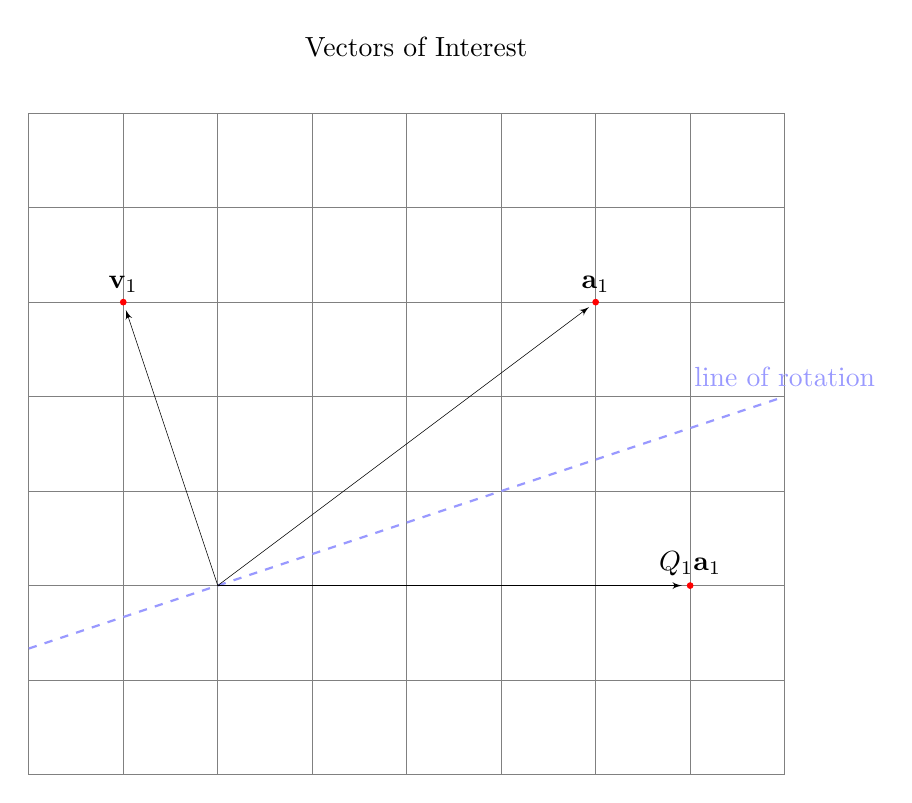
\begin{tikzpicture}[scale=1.2, vect/.style={->,shorten >=3pt,>=latex'}]
			\tkzInit[xmax=6,ymax=5,xmin=-2,ymin=-2]
			\tkzGrid
			\tkzAxeXY
			\tkzDefPoint(0, 0){O}
			\tkzDefPoint(4, 3){a1}
			\tkzDefPoint(5, 0){Q1a1}
			\tkzDefPoint(-1, 3){v1}
			\draw[blue!40,dashed,thick] (-2,-2/3) -- (6,2) node[anchor=south] {line of rotation};
			\tkzDrawPoints[color=red](a1,Q1a1,v1)
			\tkzDrawSegments[vect](O,a1 O,Q1a1 O,v1)
			\tkzLabelPoint[above](v1){$\vb{v}_1$}
			\tkzLabelPoint[above](a1){$\vb{a}_1$}
			\tkzLabelPoint[above](Q1a1){$Q_1\vb{a}_1$}
			\tkzText[above](2.1,5.5){Vectors of Interest}
		\end{tikzpicture}
	\end{center}
	I couldn't draw it on the picture, but it's worth noting that $\vb{v}_1$ is perpendicular to the line of rotation as expected.

	\ref{part:5d}
	We can now compute $Q_1A$.
	\begin{equation*}
		Q_1A = \frac{-1}{5}\mqty[4 & 3 \\ 3 & -4]\mqty[4 & 5 \\ 3 & 10] = \frac{-1}{5}\mqty[25 & 50 \\ 0 & -25] = \mqty[-5 & -10 \\ 0 & 5]
	\end{equation*}
	Thus we can write the complete $QR$ factorization as
	\begin{equation*}
		A = QR = \frac{-1}{5}\mqty[4 & 3 \\ 3 & -4]\mqty[-5 & -10 \\ 0 & 5]
	\end{equation*}
\end{solution}

\begin{problem}
Determinant inequality.
\end{problem}

\begin{solution}
	Let's start with a helpful corollary.
	\begin{corollary}
		If $x\in\mathbb{R}^n$ then $\norm{x}_\infty \leq \norm{x}_2$.
	\end{corollary}
	\begin{proof}
		\begin{equation*}
			\norm{x}_\infty = \max_i\abs{x_i} = \qty(\max_i{x_i^2})^{1/2} \leq \qty(\sum_ix_i^2)^{1/2} = \norm{x}_2
		\end{equation*}
	\end{proof}
	We'll use that in a bit, in the meantime let's return to the problem.

	Starting with the fact that $A$ is invertible, we know we can factor $A$ as $A = QR$ where $Q$ is an orthogonal matrix, and $R$ is upper triangular. Using the the fact that the determinant of product of matrices is the product of the determinants we can write $\det A = \det Q \cdot \det R$. The orthogonality of $Q$ means $\det Q = \pm 1$, and hence $\abs{\det A} = \abs{\det R}$. Since $R$ is upper triangular we know the determinant will be the product of the diagonal elements: $\det R = \prod_i r_{ii}$. Using the Gram-Schmidt version of $QR$ decomposition we know the diagonal terms are given by $\langle\vb{e}_i, \vb{a}_i\rangle$\footnote{Here we are using the convention that $\vb{e}_i$ is the vector with 1 in the $i$th spot and 0 elsewhere.} and hence $\det R = \prod_i \langle\vb{e}_i, \vb{a}_i\rangle = \prod_i (\vb{a}_i)_i$ where $(\vb{a}_i)_i$ is the $i$th component of vector $\vb{a}_i$.

	So far we have shown $\abs{\det A} = \prod_i(\vb{a}_i)_i$ so now we need to show $\prod_i(\vb{a}_i)_i \leq \prod_i\norm{\vb{a}_i}_2$. If we are able to show $(\vb{a}_i)_i \leq \norm{\vb{a}_i}_2$ is true for each $i$, then surely the product statement holds as well so we'll do that.
	\begin{equation*}
		(\vb{a}_i)_i \leq \max_j(\vb{a}_i)_j = \norm{\vb{a}_i}_\infty \leq \norm{\vb{a}_i}_2
	\end{equation*}
	With that we've shown that the $i$th component of a vector is smaller than the 2 norm of it (which sounds obvious put that way), and hence $\prod_i(\vb{a}_i)_i \leq \prod_i\norm{\vb{a}_i}_2$.

	As a recap we used the $QR$ factorization of $A$ to show $\abs{\det A} = \abs{\det R}$ and $R$'s upper triangular form to show $\abs{\det A} = \abs{\prod_i(\vb{a}_i)_i}$. We then used the corollary from above to prove
	\[
		\abs{\det A} \leq\prod_i\norm{\vb{a}_i}_2.
	\]
\end{solution}

\begin{problem}
Norm inequality.
\end{problem}

\begin{solution}
	The first thing we'll do is rewrite the inequality.
	\begin{align*}
		\frac{1}{\kappa(A)}      & \leq \frac{\norm{A - B}}{\norm{A}} \\
		\frac{1}{\norm{\inv{A}}} & \leq \norm{A - B}                  \\
		1                        & \leq \norm*{\inv{A}}\norm{A - B}
	\end{align*}
	So our goal will be to show this expression on the right is greater than one. We can use the submultiplicative property of matrix norms\footnote{$\norm{AB} \leq \norm{A}\norm{B}$.} to write $\norm{\inv{A}(A - B)} \leq \norm{\inv{A}}\norm{A- B}$. Now let's take an $x\in\ker(B)$ with $\norm{x} = 1$\footnote{This is always possible because the kernel of an operator is a subspace and hence must be amenable to scaling.} and send it through $\inv{A}(A - B)$.
	\begin{equation*}
		\inv{A}(A - B)x = \inv{A}(Ax - Bx) = \inv{A}Ax = x
	\end{equation*}
	Taking the (vector) norm of both sides yields $\norm{\inv{A}(A - B)x} = 1$. With the way the matrix norm is defined as the maximum over a set of vectors that $x$ is in, we can conclude $\norm{\inv{A}(A-B)} \geq 1$.

	Because $\norm{\inv{A}(A - B)} \leq \norm{\inv{A}}\norm{A- B}$ we can thus conclude $1\leq \norm*{\inv{A}}\norm{A - B}$ by combining these two inequalities.
\end{solution}

\end{document}
